Der Ablauf von Kaufprozessen hat sich in den letzten Jahrzehnten unter Einfluss des Onlinhandels stark geändert. Insbesondere Amazon hat sich als Händler mit niedrigen Preisen und einer sehr großen Auswahl von neuen sowie gebrauchten Produkten weltweit als Verkaufsplattform etabliert. Mithilfe dieser Kombination kann Amazon, im Gegensatz zu anderen Plattformen wie Ebay als Haupteinkaufsmöglichkeit benutzt werden, was wiederrum anderer Online-Konkurrenz und dem stationären Einzelhandel schadet. Dass Amazon insbesondere bei jungen Personen beliebt ist, konnten wir auch durch unsere Schülerumfrage am hennebergischen Gymnasium "Georg Ernst" feststellen: hier gaben 139 von 147 Teilnehmern an, bereits etwas auf Amazon gekauft zu haben.

\begin{figure}[H]
    \begin{center}
        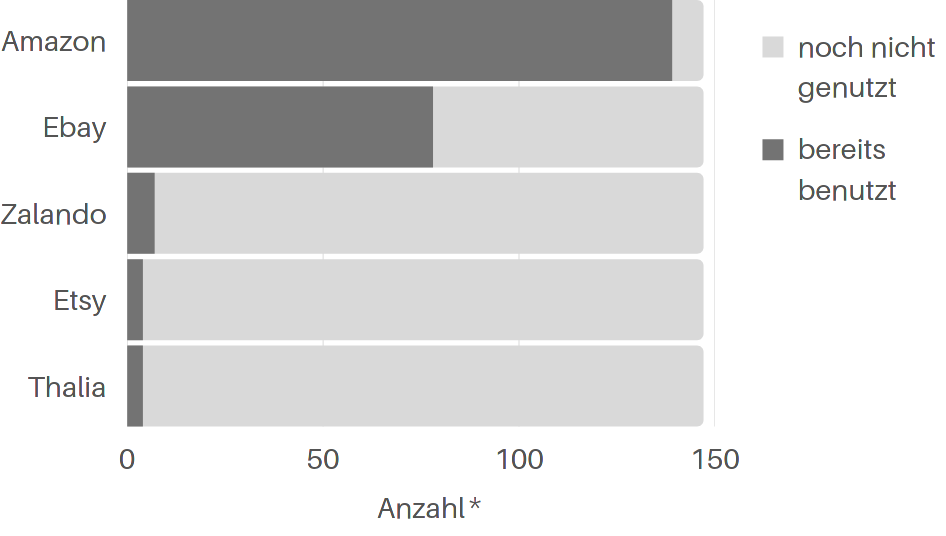
\includegraphics[width=9cm]{media/schuelerumfrage/2-cut.png} 
        \caption{Über welche Plattformen haben Sie bereits online bestellt?}
        \label{umfrage-plattformen}
        \bildquelle eigene Darstellung
    \end{center}
\end{figure}


%Neben Ebay, welches sich ausschließlich auf Drittanbieter fokussiert, konnte sich nur ein anderes Unternehmen im Onlineverkauf aller Branchen etablieren: Abiexpress, welches noch niedirgere Preise durch Direktverkauf von Herstellern ermöglicht. \emerald 345
Der Hauptgrund für diesen Wandel ist wahrscheinlich, dass bei den meisten Verbrauchsgütern die in [4] beschriebenen Vorteile des stationären Handels, hauptsächlich die Beratung und das direkte Betrachten des Produktes, nur wenig Nutzen finden\cite[S. 2]{Maier}. So ist z. B. beim wiederholten Kaufen von Shampoo, Rasierklingen o. ä. das Produkt schon bekannt und kann problemlos Online bestellt werden. 
\iffalse
    über zeit unkomplizierter geworden
    
    verbilligung des onlinehandels > prime-verlust
    amazon = vorreiter, aliexpress
    
    aliexpress: direkt von hersteller kaufen (https://www.emerald.com/insight/content/doi/10.1108/S1745-886220180000013014/full/pdf?title=italicamazon-and-alibabaitalic-internet-governance-business-models-and-internationalization-strategies 345)
\fi
Dementsprechend führt die seit Jahrzehnten steigende Relevanz des Onlinehandels zu einem Rückgang der Nachfrage im stationären Vertrieb\cite{Shankar}, die durch die derzeitige Corona-Situation noch etwas verstärkt wird - mehr dazu in Kapitel [4 und 5].

\iffalse
 Vorreiter in sachen niedrige Preise > ist sehr wichtig, weil
   viel einfacher vergelichbar, qualität des Produkts nicht einfach einsehbar: sie muss nicht außergewöhnlich, nur akzeptabel sein - jedoch auch nicht schlecht, da 14-tage-rückgabe ohne angabe eines grundes

 
 S 49 https://edoc.sub.uni-hamburg.de/hcu/volltexte/2017/370/pdf/Ebert_Kirsten.pdf
 danach: modell für veränderung
\fi
